% =====================================================================
%  CITIS 2026 submission -- Springer LNNS (LLNCS) proceedings template.
%  DOUBLE-BLIND: author/affiliation/identifying info removed from the body.
%
%  CAMERA-READY AUTHOR BLOCK (do NOT include in the blind submission):
%    Roberto Hincapie, Roy Sandoval
%    Ingenieria en Ciencia de Datos, Universidad Pontificia Bolivariana, 2026
% =====================================================================
\documentclass[runningheads]{llncs}

\usepackage[T1]{fontenc}
\usepackage[utf8]{inputenc}
\usepackage{amsmath,amssymb}
\usepackage{graphicx}
\usepackage{booktabs}
\usepackage{algorithm}
\usepackage{algpseudocode}
\usepackage{url}

\begin{document}

\title{Capacitated School Bus Routing via Clustering and
Network-Based Optimization: A Comparative Benchmark of Six Strategies
on a Real Road Network}

\titlerunning{Capacitated School Bus Routing: A Comparative Benchmark}

% --- Anonymized for double-blind review ---
\author{Anonymous Author(s)}
\authorrunning{Anonymous}
\institute{Anonymized for double-blind review}

\maketitle

\begin{abstract}
The School Bus Routing Problem (SBRP) is an NP-hard combinatorial
optimization problem that generalizes the capacitated vehicle routing
problem and underpins a service used daily by millions of students.
Although the literature offers many heuristic and metaheuristic
strategies, head-to-head comparisons under identical, realistic
conditions remain scarce, which makes it difficult for practitioners
to choose a method. We present a unified benchmark that evaluates six
clustering- and covering-based routing strategies---capacitated
k-medoids, a multi-objective sectorial clustering, a zonal
capacitated vehicle routing problem with time windows (CVRPTW), two
set-covering integer programs, and a genetic algorithm---on identical
scenarios generated from the real OpenStreetMap road network of
Medell\'in (Colombia). All methods share a common solver interface,
directed shortest-path distances, a single depot, and a bus capacity
of twenty, and are measured on fleet distance, computation time,
fleet size, coverage and cluster cohesion across student densities
$N\in\{50,100,200,400\}$ with eleven seeds each (264 runs). A Friedman
test confirms that the strategies differ significantly in both fleet
distance ($p<10^{-34}$) and latency ($p<10^{-32}$). Capacitated
k-medoids and sectorial clustering are statistically tied for the
shortest fleet distance (Wilcoxon $p=0.36$), while set-covering
formulations are orders of magnitude faster at a quality cost, and the
one genetic encoding we test---a flat permutation with a positional
capacity decoder---degrades sharply with scale. We distill the
trade-offs into practical guidance for SBRP solver selection.

\keywords{School Bus Routing Problem \and Capacitated clustering
\and Vehicle routing \and Metaheuristics \and Set covering
\and Road-network optimization.}
\end{abstract}

% =====================================================================
\section{Introduction}
% =====================================================================
The School Bus Routing Problem (SBRP) consists of planning a fleet of
buses that collects students from a set of stops and delivers them to
their school while respecting operational constraints such as vehicle
capacity, maximum riding time and bell-time windows~\cite{Park2010TheReview}.
It is a generalization of the capacitated vehicle routing problem
(CVRP), which itself descends from the truck-dispatching problem first
formalized by Dantzig and Ramser~\cite{DantzigRamser1959Truck}, and it
is therefore NP-hard. The intractability is also combinatorial: a bus
visiting $n_c$ stops admits $n_c!$ visiting orders, and the partition
of students across buses must be chosen jointly with those orders, so
naive enumeration grows factorially in the number of stops. Both facts
point the same way---exact methods are infeasible at realistic $n$.
As a result, practical SBRP
solvers are overwhelmingly heuristic, and the survey by Park and
Kim~\cite{Park2010TheReview} together with the more recent review of
Ellegood et al.~\cite{Ellegood2020SchoolDirections} shows that the
field is fragmented into many problem variants and solution paradigms
whose relative merits are rarely measured on common ground.

A classical and still dominant family of heuristics follows the
\emph{cluster-first, route-second} paradigm: students are first
grouped into capacity-feasible clusters, and a Traveling Salesman
Problem (TSP) is then solved within each cluster, for which highly
effective heuristics exist---notably Croes' 2-opt local
search~\cite{Croes1958TwoOpt} and Helsgaun's implementation of the
Lin--Kernighan heuristic~\cite{HelsgaunAnHeuristic}.
The clustering step can be guided by geometry~\cite{CakirRevisitingProblem},
by classical partitioning algorithms~\cite{Comert2018AStudy}, or by
multiple and often conflicting objectives such as simultaneously
minimizing the number of buses and the students' riding
time~\cite{Corberan2002HeuristicObjectives}. An orthogonal family
formulates route selection directly as a set-covering integer
program, and a third relies on population-based metaheuristics such as
genetic, annealing or nature-inspired
algorithms~\cite{Baranwal2016DAVRPTW,Hatamlou2018BlackHole}.

The difficulty for a practitioner is that these strategies are
typically published on different instances, with different distance
models (Euclidean vs.\ road network), different objectives and
different computational budgets, so their reported numbers cannot be
compared directly. This paper addresses that gap. Our contributions
are:

\begin{itemize}
\item A \textbf{unified benchmark harness} exposing six SBRP strategies
through one interface and evaluating them on \emph{identical} scenarios
built from the real road network of Medell\'in and the Valle de
Aburr\'a, under the same capacity, distance model and metrics.
\item A \textbf{rigorous description} of each strategy: a formal
decision-variable model, and worst-case complexity checked against
\emph{measured} per-stage cost.
\item A \textbf{statistically grounded comparison} across four densities
and eleven seeds (264 runs), using Friedman and Wilcoxon tests with a
Nemenyi post-hoc to separate genuine differences from noise.
\item \textbf{Practical guidance}: capacitated k-medoids and sectorial
clustering are statistically tied for the best fleet distance,
set-covering programs are the speed/coverage sweet spot, and a
topology-agnostic genetic encoding scales poorly---with an explanation
of \emph{why}.
\end{itemize}

\paragraph{Relevance to data-driven urban planning.}
This work addresses \emph{smart mobility and data-driven urban
planning}: it decides school transport from the real street topology of a
metropolitan area, and re-targets to another city by swapping the graph
and service polygons. Total fleet distance is exactly the
vehicle-kilometres travelled (VKT) that drives fuel use, emissions and
congestion, so the spread between solvers is not merely algorithmic: at
$N=400$ the worst commits $1006$~km against $460$~km for the best, a
$2.2\times$ VKT difference for the same students, buses and network. We
stop at VKT deliberately---converting it to emissions needs
fleet-specific factors we lack for the study area, so that step and
validation against municipal operations are future work, not an estimate
we invent~\cite{Sabet2022GreenVRP}.

% =====================================================================
\section{Related Work}\label{sec:related}
% =====================================================================
\subsection{The School Bus Routing Problem}
The SBRP has been studied for almost five decades. Park and
Kim~\cite{Park2010TheReview} decompose it into five sub-problems---data
preparation, bus-stop selection, route generation, route scheduling
and bell-time adjustment---and observe that most contributions tackle
one or two of these in isolation. The updated survey of Ellegood et
al.~\cite{Ellegood2020SchoolDirections} reviews 64 newer publications
and confirms that single-school, capacity-constrained route generation
remains the most studied core, and that heuristic and metaheuristic
methods dominate exact ones in practice. The most recent synthesis, by
Wang et al.~\cite{Wang2025SBRPReview}, covers the literature through
2024 and records a shift from single-objective cost minimization towards
multi-objective formulations adding heterogeneous fleets, service equity
and dynamic constraints, alongside marked growth in metaheuristic and
learning-based methods---while noting what motivates this paper: the
proliferation of variants has outpaced comparative evaluation.
Corber\'an et
al.~\cite{Corberan2002HeuristicObjectives} emphasize the inherently
\emph{multi-objective} nature of the problem: minimizing the number of
buses and minimizing student travel time are conflicting goals, and a
good solver must navigate that trade-off rather than optimize a single
scalar. Our benchmark adopts the single-school, capacitated, route-generation
variant and reports several of these competing objectives side by side.

\subsection{Cluster-first, route-second}
Clustering was central to early VRP algorithms and has seen renewed
interest. Cakir et al.~\cite{CakirRevisitingProblem} revisit
cluster-first, route-second with a shape-based clustering that forms
clusters of a desired geometry relative to the depot, which is the
conceptual ancestor of our sectorial strategy. Comert et
al.~\cite{Comert2018AStudy} solve a capacitated VRP by first
partitioning customers with k-means, k-medoids or random clustering
and then routing each cluster, and report that medoid-based clustering
yields the most robust routes---a finding our results corroborate on a
real road network. The k-medoids/PAM family itself originates with
Kaufman and Rousseeuw~\cite{KaufmanRousseeuw1990PAM}, and we use the
FasterPAM variant for initialization. Geometry- and curve-based
clustering continues to advance, e.g.\ the sub-trajectory set-cover
formulation of Akitaya et al.~\cite{Akitaya2021Subtrajectory}, which
also links clustering to set covering---the two paradigms we contrast.

\subsection{Routing and metaheuristics}
Within a cluster, route construction reduces to the TSP. The savings
heuristic of Clarke and Wright~\cite{ClarkeWright1964Savings} and local
search such as 2-opt~\cite{Croes1958TwoOpt} are the classical building
blocks, while the Lin--Kernighan heuristic and its
implementations~\cite{HelsgaunAnHeuristic} remain the state of the art
for high-quality tours. Modern solvers wrap these in metaheuristics;
Google OR-Tools~\cite{PerronFurnon2023ORTools}, which we use for the
routing stage, drives local search with Guided Local
Search~\cite{Voudouris1999GLS}. Population- and physics-inspired
metaheuristics are also widely applied to routing: deterministic
annealing for the VRP with time windows~\cite{Baranwal2016DAVRPTW},
the black-hole algorithm for the TSP~\cite{Hatamlou2018BlackHole}, and
genetic algorithms~\cite{Holland1992Adaptation}. More recently,
learning-based approaches such as graph convolutional networks have
been proposed for the TSP~\cite{Joshi2019GCN,Dahiya2018TSPReview}, and
neural combinatorial optimization has matured into a distinct family of
VRP solvers~\cite{Wu2024NCOSurvey}. A parallel line makes
sustainability an explicit objective, formulating emissions- and
energy-aware ``green'' VRP variants~\cite{Sabet2022GreenVRP}. We include a
genetic algorithm as a deliberately simple representative of the
metaheuristic family and analyze why a topology-agnostic encoding
underperforms the clustering pipelines at scale; the learned and hybrid
approaches are outside our scope and we do not claim to bound them.

% =====================================================================
\section{Methods}\label{sec:methods}
% =====================================================================
This section presents the methods in three parts: the formal problem
statement (Section~\ref{sec:problem}), the six solution strategies with
their models and complexity (Sections~\ref{sec:framework}--\ref{sec:complexity}),
and the experimental protocol (Section~\ref{sec:setup}).

\subsection{Problem formulation}\label{sec:problem}
\subsubsection{Notation and distances.}
Let the road network be a directed weighted graph $G=(V,E)$ with arc
weights $w_e>0$. A single school (depot) $o\in V$ and a set of
$n$ student stops $\mathcal{C}=\{1,\dots,n\}\subset V$ are given,
together with a homogeneous fleet of buses of capacity $C$. For any
pair $i,j\in V$ the road distance is the shortest-path cost
\begin{equation}
d_{ij}=\min_{p\in\mathcal{P}(i,j)}\sum_{e\in p} w_e ,
\end{equation}
where $\mathcal{P}(i,j)$ is the set of directed paths from $i$ to $j$;
distances are in general asymmetric ($d_{ij}\neq d_{ji}$). Clustering
algorithms that assume a metric use the symmetrized matrix
\begin{equation}
D^{\mathrm{sym}}_{ij}=\tfrac{1}{2}\,(d_{ij}+d_{ji}) ,
\end{equation}
whereas the routing stage uses the directed distances $d_{ij}$.

\subsubsection{Objective and constraints.}
The SBRP we address is a single-depot CVRP. A solution is a set of
closed routes, one per bus, each starting and ending at $o$. The
number of buses is lower-bounded by
$k=\lceil n/C\rceil$. The objective is to minimize the total fleet
distance
\begin{equation}
L_{\mathrm{total}}=\sum_{c}\sum_{(i,j)\in r_c} d_{ij}\,,
\label{eq:obj}
\end{equation}
subject to: (i)~every student is served by exactly one bus (full
coverage); (ii)~no route carries more than $C$ students; and
(iii)~every route starts and ends at the depot. Because solving this
CVRP exactly is intractable, we adopt the cluster-first, route-second
decomposition into a capacitated assignment sub-problem followed by
$k$ independent TSPs.

Constraint~(i) is hard for five of the six strategies. The zonal CVRPTW
is the exception: it also enforces a route-duration limit, which can
conflict with coverage on peripheral stops, so it relaxes~(i) to
$\sum_{c} x_{ic}+u_i=1$ with $u_i\in\{0,1\}$ marking student $i$
unserved and adds $\Pi\sum_i u_i$ to the objective, for $\Pi$ large
enough that a drop is worse than any feasible detour
(Section~\ref{sec:cvrptw}). Coverage is reported as a first-class
metric so this relaxation stays visible in every comparison.

\subsubsection{Capacitated assignment sub-problem.}
Given current cluster representatives (medoids)
$M=\{m_1,\dots,m_k\}$, the assignment of students to clusters is the
binary program
\begin{align}
\min \quad & \sum_{i=1}^{n}\sum_{c=1}^{k} D^{\mathrm{sym}}_{i,m_c}\,x_{ic}
\label{eq:assign-obj}\\
\text{s.t.}\quad & \sum_{c=1}^{k} x_{ic}=1 \quad \forall i, \label{eq:assign-cover}\\
& \sum_{i=1}^{n} x_{ic}\le C \quad \forall c, \label{eq:assign-cap}\\
& x_{ic}\in\{0,1\},
\end{align}
where $x_{ic}=1$ iff student $i$ joins cluster $c$. As the constraint
matrix of (\ref{eq:assign-obj})--(\ref{eq:assign-cap}) is totally
unimodular, the program is solved to optimality as a minimum-cost flow
in a four-layer network (source~$\to$~students~$\to$~medoids~$\to$~sink),
avoiding a general integer solver. Each cluster's medoid is then
recomputed as the within-cluster $1$-median
$m_c=\arg\min_{h\in S_c}\sum_{i\in S_c} D^{\mathrm{sym}}_{ih}$, and the
two steps alternate until the medoids stabilize.

\subsubsection{Per-cluster routing sub-problem.}
For cluster $c$ with node set $V_c=S_c\cup\{o\}$ and binary arc
variables $y_{ij}$, the route is the TSP tour
\begin{align}
\min \quad & \sum_{(i,j)\in V_c\times V_c} d_{ij}\,y_{ij}\\
\text{s.t.}\quad & \textstyle\sum_{j\neq i} y_{ij}=1,\;\;
\sum_{i\neq j} y_{ij}=1 \quad \forall i,j\in V_c,\\
& \textstyle\sum_{i\in S}\sum_{j\in S} y_{ij}\le |S|-1
  \quad \forall\, S\subsetneq V_c,\; 2\le|S|\le|V_c|-1,
  \label{eq:dfj}\\
& y_{ij}\in\{0,1\},
\end{align}
where (\ref{eq:dfj}) is the Dantzig--Fulkerson--Johnson
subtour-elimination family: forbidding any proper subset $S$ from
carrying $|S|$ internal arcs rules out cycles that do not span $V_c$.
Having exponentially many members, it is not enumerated: OR-Tools
maintains a single connected circuit by construction and improves it
with Guided Local Search~\cite{Voudouris1999GLS} under a fixed budget,
so (\ref{eq:dfj}) defines the optimum we approximate, not the algorithm.

\subsubsection{Set-covering formulation.}
An alternative that bypasses explicit clustering enumerates a pool
$\mathcal{R}$ of capacity-feasible candidate routes and selects a
subset. Minimizing the number of buses gives the set-cover program
\begin{equation}
\min \sum_{j\in\mathcal{R}} x_j \quad\text{s.t.}\quad
\sum_{j:\,i\in R_j} x_j \ge 1\;\;\forall i\in\mathcal{C},\quad
x_j\in\{0,1\},
\label{eq:setcover}
\end{equation}
while replacing the objective by $\sum_j \mathrm{cost}_j\,x_j$ (the
route length) minimizes distance instead. Both variants are solved
with a branch-and-cut integer solver.

\subsection{Common benchmark framework}\label{sec:framework}
All strategies are implemented as adapters behind a single
\texttt{Solver} interface: each receives a \texttt{Scenario} (the same
road graph, student locations, depot and capacity) and returns a
\texttt{Solution} (a list of closed routes and, optionally, cluster
labels). This guarantees that the six methods are evaluated on
byte-identical inputs and scored by the same metric code, removing
instance and implementation bias from the comparison. The framework is
written in Python and relies on OSMnx~\cite{Boeing2017OSMnx} for
road-network extraction, NetworkX for graph algorithms and minimum-cost
flow, OR-Tools~\cite{PerronFurnon2023ORTools} for TSP/CVRPTW search,
FasterPAM~\cite{KaufmanRousseeuw1990PAM} for medoid initialization, a
branch-and-cut integer solver (CBC) for the set-covering programs, and
scikit-learn~\cite{Pedregosa2011Sklearn} for the silhouette score. The
scenario generator is deterministic given the pair $(N,\text{seed})$, so
every instance is reproducible.

\subsection{Capacitated k-medoids + OR-Tools (baseline)}
The baseline instantiates the cluster-first, route-second
decomposition exactly as formalized above (Algorithm~\ref{alg:kmedoids}):
FasterPAM provides initial medoids, the capacitated assignment is
solved by minimum-cost flow, medoids are recomputed, and the loop
iterates to convergence before each cluster is routed with OR-Tools.

\begin{algorithm}[t]
\caption{Capacitated k-medoids + per-cluster TSP}
\label{alg:kmedoids}
\footnotesize
\begin{algorithmic}[1]
\Require symmetrized distances $D^{\mathrm{sym}}$, directed distances $d$,
capacity $C$, depot $o$, iteration cap $T$
\State $k \gets \lceil n/C\rceil$
\State $M \gets \textsc{FasterPAM}(D^{\mathrm{sym}},k)$ \Comment{initial medoids}
\Repeat
  \State $x \gets \textsc{MinCostFlowAssign}(D^{\mathrm{sym}},M,C)$
         \Comment{Eqs.~(\ref{eq:assign-obj})--(\ref{eq:assign-cap})}
  \ForAll{clusters $S_c$}
     \State $m_c \gets \arg\min_{h\in S_c}\sum_{i\in S_c} D^{\mathrm{sym}}_{ih}$
  \EndFor
\Until{$M$ unchanged \textbf{or} $T$ iterations}
\ForAll{clusters $S_c$}
  \State $r_c \gets \textsc{OrToolsTSP}(S_c\cup\{o\},d)$ \Comment{Guided Local Search}
\EndFor
\State \Return $\{r_c\}$
\end{algorithmic}
\end{algorithm}

\subsection{Sectorial multi-objective clustering}
The sectorial strategy replaces the
purely distance-driven assignment by a geometric one inspired by
shape-based clustering~\cite{CakirRevisitingProblem}. Each student is
scored by a convex combination of its angular position and its radial
distance with respect to the school,
\begin{equation}
s_i=\alpha\,\frac{\theta_i+\pi}{2\pi}+\beta\,\hat d_i,
\qquad \alpha+\beta=1,
\label{eq:sectorial-score}
\end{equation}
where $\theta_i=\operatorname{atan2}(y_i-y_o,\,x_i-x_o)$ and
$\hat d_i$ is the min--max-normalized distance to the depot
($\alpha=0.6,\beta=0.4$ by default). An angular sweep packs students
into capacity-bounded sectors, which are then refined with the same
minimum-cost-flow reassignment as the baseline, optionally penalizing
moves that break the initial sweep. The result is a set of compact,
wedge-shaped clusters that radiate from the school.


\subsection{Zonal CVRPTW}\label{sec:cvrptw}
This strategy partitions the metropolitan area into six fixed
geographic zones (communes and municipalities of the Valle de
Aburr\'a, by point-in-polygon test) and solves an independent CVRPTW
per zone with OR-Tools. Beyond capacity it enforces a time dimension:
travel time plus a $90$-second boarding time per stop, a maximum route
duration of $75$ minutes, and a span-balancing penalty that
discourages long routes. Unserved stops are allowed at a high penalty,
so the method can leave a small fraction of students uncovered when the
duration limit binds.

Formally, with $Z$ indexing zones, $\mathcal{C}_z$ the students inside
zone $z$, binary arc variables $y^z_{ij}$, drop indicators
$u_i\in\{0,1\}$ and arrival times $a_i\ge0$, each zone solves
\begin{align}
\min \;\; & \sum_{z\in Z}\Big[\sum_{(i,j)} d_{ij}\,y^z_{ij}
  + \gamma\,\sigma_z\Big] + \Pi\sum_{i\in\mathcal{C}} u_i
\label{eq:cvrptw}\\
\text{s.t.}\;\; & \textstyle\sum_{j} y^z_{ij} = 1-u_i,\quad
\sum_{i\in r} q_i \le C,\quad
a_j \ge a_i + \tau_{ij} + b,
\nonumber
\end{align}
plus $a_{\text{end}}-a_{\text{start}}\le T_{\max}$ per route, with
$\tau_{ij}$ directed travel time, $b=90$~s boarding, $T_{\max}=75$~min,
$\sigma_z$ the duration span penalized by $\gamma$, and $\Pi$ the drop
penalty of Section~\ref{sec:problem}. The constraint
$\sum_j y^z_{ij}=1-u_i$ is the soft-coverage relaxation: a student is
visited once or dropped at cost $\Pi$, and since $\Pi$ dominates any
routing saving, drops arise only where the duration limit admits no
feasible insertion. With a single bell time the time windows reduce to
that limit, which is what binds here.

\subsection{Set-covering integer programs}
Two variants instantiate the set-cover model of
Eq.~(\ref{eq:setcover}). The \emph{per-child} variant builds one
candidate route per student by greedily packing its $C-1$ nearest
neighbors, then selects the minimum number of routes covering all
students. The \emph{grid} variant seeds candidates on a Cartesian grid
whose spacing scales with student density, builds a greedy tour around
each seed, and selects routes minimizing total distance subject to full
coverage. Both are solved by branch-and-cut.

The two variants differ only in how the pool $\mathcal{R}$ and the
objective coefficients of Eq.~(\ref{eq:setcover}) are instantiated.
Per-child builds $\mathcal{R}=\{R_1,\dots,R_n\}$ with
$R_i=\{i\}\cup\mathrm{NN}_{C-1}(i)$, the $C-1$ nearest neighbours of
$i$ under $D^{\mathrm{sym}}$, giving $|\mathcal{R}|=n$ candidates in
$O(n^2)$ time, and minimizes $\sum_j x_j$ (fleet size). Grid overlays a
Cartesian lattice whose spacing shrinks with student density, and for
each occupied cell greedily grows one capacity-feasible route around
the cell seed; the objective becomes
$\sum_j \mathrm{cost}_j x_j$ with $\mathrm{cost}_j$ the length of a
greedy tour over $R_j$.

Two properties explain most of these variants' quality gap.
Eq.~(\ref{eq:setcover}) is a \emph{covering} ($\ge1$), not
\emph{partitioning} ($=1$), constraint and the selected routes run as
generated, so a student in two selected candidates is visited twice and
both visits are charged: at $N=400$ per-child selects $26.9$
capacity-filled routes---$538$ seats for $400$ students---making about a
quarter of visits redundant. Their distances are thus the cost of a
covering plan, not a partition. Second, $\mathcal{R}$ is a heuristically
seeded subset of all $\binom{n}{\le C}$ feasible routes, so speed comes
from the small pool, not from branch-and-cut being easy.

\subsection{Genetic algorithm}
The genetic algorithm (Algorithm~\ref{alg:ga}) represents a solution as
a permutation of the $n$ students. A capacity-aware decoder splits the
permutation into consecutive chunks of at most $C$ students and routes
each chunk with a nearest-neighbor construction followed by a single
2-opt~\cite{Croes1958TwoOpt} pass; the fitness is the resulting total
fleet distance. Evolution uses tournament selection, order crossover
(OX), swap mutation and elitism, and stops at a generation cap or after
a stagnation window.

\begin{algorithm}[t]
\caption{Genetic algorithm with capacity-aware decoder}
\label{alg:ga}
\footnotesize
\begin{algorithmic}[1]
\Require capacity $C$, population $P$, generations $G$, mutation rate
$p_m$, tournament size $t$, elites $e$
\State initialize $P$ random permutations of $\{1,\dots,n\}$
\State evaluate each via \textsc{Decode} (split by $C$; per chunk: NN $+$ 2-opt; sum $d$)
\For{$g=1$ to $G$}
  \State carry the $e$ best individuals (elitism)
  \While{next generation incomplete}
    \State $p_1,p_2 \gets \textsc{Tournament}(t)$
    \State $\textit{child} \gets \textsc{OX-Crossover}(p_1,p_2)$
    \If{$\mathrm{rand}()<p_m$} $\textit{child}\gets\textsc{SwapMutation}(\textit{child})$ \EndIf
  \EndWhile
  \State evaluate offspring; \textbf{if} no improvement for $S$ generations \textbf{then break}
\EndFor
\State \Return best decoded solution
\end{algorithmic}
\end{algorithm}

\subsection{Complexity analysis}\label{sec:complexity}
Table~\ref{tab:complexity} summarizes each strategy's asymptotic
worst-case cost alongside the stage that actually dominates its measured
runtime, where $n$ is the number of students, $k=\lceil n/C\rceil$ the
number of buses, $T$ the iteration cap, $P$ the population and $G$ the
generations. The distinction matters, because for the two flow-based
pipelines the asymptotically expensive stage is \emph{not} the one that
governs the wall-clock times in Section~\ref{sec:results}.

We timed the stages rather than assuming which dominates. For K-medoids
and Sectorial the minimum-cost-flow assignment takes $0.04\%$ of solver
time at $N=50$ and only $1.1\%$ at $N=400$ ($1.09$ of $101.13$~s), with
FasterPAM under $0.02$~s; the per-cluster TSP takes the remaining
$98.9$--$99.96\%$ and is \emph{budget-bound}, costing almost exactly
$k\cdot B$ ($15.03$, $25.01$, $50.01$, $100.03$~s for $k=3,5,10,20$ at
$B=5$~s). As $k=\lceil n/C\rceil$, latency grows \emph{linearly} in $n$,
as Table~\ref{tab:latency} shows. The $O(T\,n^3)$ flow bound is real but
latent---its share rises two orders of magnitude from $N=50$ to
$N=400$---so it dominates only far beyond the sizes studied.

\begin{table}[t]
\centering
\caption{Asymptotic worst-case cost per strategy, and the stage that
dominates the \emph{measured} runtime, from per-stage timers at $N{=}400$
($B$ = per-cluster TSP budget, $5$~s; $B_z$ = per-zone CVRPTW budget,
$20$~s). $^\dagger$~inferred from latency being invariant in $n$, not timed.}
\label{tab:complexity}
\small
\setlength{\tabcolsep}{4pt}
\begin{tabular}{lll}
\toprule
\textbf{Strategy} & \textbf{Asymptotic worst case} &
\textbf{Measured dominant stage}\\
\midrule
K-medoids + TSP & $O(T\,n^3)$, min-cost flow & TSP budget $k\,B$ ($98.9\%$)\\
Sectorial       & $O(T\,n^3)$, sweep $+$ flow & TSP budget $k\,B$ ($99.0\%$)\\
CVRPTW (zonal)  & $O(n^2)$--$O(n^3)$, GLS & zone budget $|Z|\,B_z^{\;\dagger}$\\
Set Cover (per-child) & ILP, exp.; $O(n^2)$ pool & ILP $67\%$, pool $28\%$\\
Set Cover (grid)      & ILP, exp.; $O(n)$ seeds & ILP ($>98\%$)\\
Genetic & $O(P\,G\,n^2)$, decoding & decoding $73\%$, operators $25\%$\\
\bottomrule
\end{tabular}
\end{table}

\subsection{Experimental setup}\label{sec:setup}
Scenarios are generated on the real drivable road network of
Medell\'in and the Valle de Aburr\'a, extracted from OpenStreetMap with
OSMnx~\cite{Boeing2017OSMnx} and restricted to the largest strongly
connected component. The depot is fixed at a university campus, and
$N$ student stops are sampled uniformly from graph nodes lying inside
the union of the six service-zone polygons, so that all instances stay
within the actual metropolitan footprint. Directed shortest-path
distance and travel-time matrices are precomputed with Dijkstra's
algorithm. The bus capacity is $C=20$.

We sweep four student densities $N\in\{50,100,200,400\}$ with eleven
seeds each, giving $44$ scenarios and $264$ runs ($6$ strategies
$\times\,44$). For every run we record: total fleet distance, wall-clock
latency, number of buses used, coverage (fraction of students served),
the silhouette coefficient~\cite{Rousseeuw1987Silhouettes} of the
clustering on the symmetrized distances, capacity violations, and the
longest single-route distance. To keep latency comparable, the
per-cluster TSP search is capped at $5$~s and the per-zone CVRPTW
search at $20$~s.

All strategies run at fixed settings across the sweep, with no
per-instance tuning, so the comparison reflects out-of-the-box
behaviour. K-medoids uses iteration cap $T=50$; Sectorial uses
$\alpha=0.6$, $\beta=0.4$, min--max radial normalization and $T=5$;
the zonal CVRPTW uses $75$~min maximum duration, $90$~s boarding and a
span-balancing coefficient of $300$. The genetic algorithm uses
$P=100$, $G=200$, $p_m=0.1$, $t=3$, $e=2$ and $S=30$; order crossover
is applied to every offspring, so there is no separate crossover rate,
and the decoder's 2-opt is limited to one pass per chunk.
Statistical significance across strategies is
assessed with the non-parametric Friedman test (blocks $=$ the $44$
scenarios), and pairwise differences with the Wilcoxon signed-rank
test.

% =====================================================================
\section{Results}\label{sec:results}
% =====================================================================
Table~\ref{tab:fleet} reports fleet distance and latency, and
Table~\ref{tab:quality} the remaining quality metrics at the most
demanding density ($N=400$). Figures~\ref{fig:scalability}
and~\ref{fig:pareto} show how latency scales and the distance--latency
trade-off; Figure~\ref{fig:grid} contrasts the solution paradigms on a
shared scenario.

\begin{table}[t]
\centering
\caption{Total fleet distance (km, mean $\pm$ std over 11 seeds) and
latency (s, mean). Bold: distance minimum among full-coverage methods.}
\label{tab:fleet}
\label{tab:latency}
\setlength{\tabcolsep}{2.2pt}
\footnotesize
\begin{tabular}{l@{\hskip 4pt}cccc@{\hskip 7pt}cccc}
\toprule
& \multicolumn{4}{c@{\hskip 10pt}}{\textbf{Fleet distance (km)}}
& \multicolumn{4}{c}{\textbf{Latency (s)}}\\
\cmidrule(r){2-5}\cmidrule{6-9}
\textbf{Strategy} & $50$ & $100$ & $200$ & $400$
                  & $50$ & $100$ & $200$ & $400$\\
\midrule
K-medoids + TSP      & \textbf{105$\pm$5}  & \textbf{163$\pm$18} & \textbf{271$\pm$21} & \textbf{460$\pm$26}
  & 15.0 & 25.0 & 50.2 & 101.0\\
Sectorial            & 105$\pm$5  & 165$\pm$19 & 272$\pm$21 & 461$\pm$25
  & 15.0 & 25.0 & 50.2 & 101.0\\
CVRPTW (zonal)$^\ast$ & 125$\pm$7  & 182$\pm$12 & 286$\pm$16 & 471$\pm$13
  & 100.0 & 100.0 & 100.0 & 100.0\\
Set Cover (per-child) & 160$\pm$27 & 254$\pm$36 & 389$\pm$39 & 670$\pm$20
  & 0.02 & 0.02 & 0.04 & 0.16\\
Set Cover (grid)      & 134$\pm$8  & 217$\pm$22 & 349$\pm$26 & 594$\pm$33
  & 0.27 & 0.74 & 3.19 & 66.6\\
Genetic               & 115$\pm$7  & 210$\pm$19 & 457$\pm$19 & 1006$\pm$30
  & 5.76 & 21.2 & 44.5 & 106.7\\
\bottomrule
\end{tabular}
\\[3pt]
{\footnotesize $^\ast$ CVRPTW may leave ${\sim}1\%$ of students unserved
when the duration limit binds, so its distance is not strictly comparable
to the full-coverage methods.}
\end{table}

\begin{table}[t]
\centering
\caption{Quality metrics at $N{=}400$, mean over 11 seeds.}
\label{tab:quality}
\small
\begin{tabular}{lcccc}
\toprule
\textbf{Strategy} & \textbf{Buses} & \textbf{Coverage} & \textbf{Silhouette} & \textbf{Max route (km)}\\
\midrule
K-medoids + TSP      & 20.0 & 1.000 & \textbf{0.276} & 46.2\\
Sectorial            & 20.0 & 1.000 & 0.266 & 45.2\\
CVRPTW (zonal)       & 22.4 & 0.998 & 0.272 & \textbf{30.3}\\
Set Cover (per-child) & 26.9 & 1.000 & 0.230 & 50.8\\
Set Cover (grid)      & 23.2 & 1.000 & 0.199 & 56.6\\
Genetic               & 20.0 & 1.000 & $-0.192$ & 79.3\\
\bottomrule
\end{tabular}
\end{table}

\paragraph{Statistical significance.}
The Friedman test rejects the null hypothesis of equal performance
across the six strategies for both fleet distance
($\chi^2=172.9$, $\mathrm{df}=5$, $p<10^{-34}$) and latency
($\chi^2=161.6$, $\mathrm{df}=5$, $p<10^{-32}$). On fleet distance the
mean ranks (1 = best) are $1.63$ for Sectorial and $1.67$ for
K-medoids, $2.93$ for CVRPTW, $4.50$ for Set Cover (grid), $4.82$ for
Genetic and $5.45$ for Set Cover (per-child). The two leaders are
statistically indistinguishable: a Wilcoxon signed-rank test between
K-medoids and Sectorial over the $44$ scenarios yields $p=0.36$. On latency the
ranking is reversed at the top---Set Cover (per-child) is fastest in
every scenario (mean rank $1.00$), followed by Set Cover (grid)
($2.16$)---confirming the quality/speed tension visible in
Figure~\ref{fig:pareto}.

Since a Friedman rejection only says \emph{some} strategies differ, we
add the Nemenyi post-hoc~\cite{Demsar2006Statistical}, which separates
two strategies when their mean ranks differ by more than
$\mathrm{CD}=q_\alpha\sqrt{k(k+1)/6N}$. With $k=6$, $N=44$,
$\alpha=0.05$ ($q_\alpha=2.850$), $\mathrm{CD}=1.14$ and $11$ of $15$
pairs clear it on distance: both leaders separate from Set Cover
(per-child) ($\Delta=3.78$--$3.83$), Genetic ($3.15$--$3.19$), Set Cover
(grid) ($2.83$--$2.88$) and the CVRPTW itself ($1.26$--$1.31$), which in
turn separates from all three trailing methods. Only four pairs remain
unresolved: K-medoids versus Sectorial ($0.045$) and the three trailing
methods among themselves ($0.32$--$0.96$).

\begin{figure}[t]
\centering
\begin{minipage}[t]{0.49\textwidth}
  \centering
  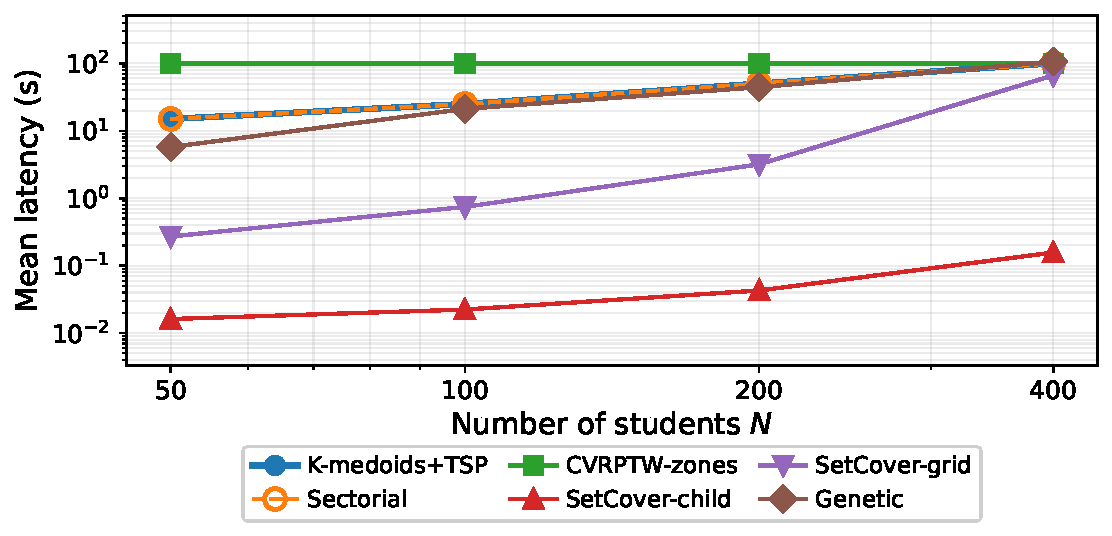
\includegraphics[width=\textwidth]{figures/scalability.pdf}
  \caption{Mean latency vs.\ $N$ (log--log). Clustering pipelines grow
  linearly in the number of buses because each is routed under a fixed
  per-cluster TSP budget; the flow assignment contributes at most
  $1.1\%$ of their runtime. K-medoids and Sectorial have near-identical
  latencies, so Sectorial is dashed with hollow markers over the solid
  K-medoids curve---both series are present throughout.}
  \label{fig:scalability}
\end{minipage}\hfill
\begin{minipage}[t]{0.49\textwidth}
  \centering
  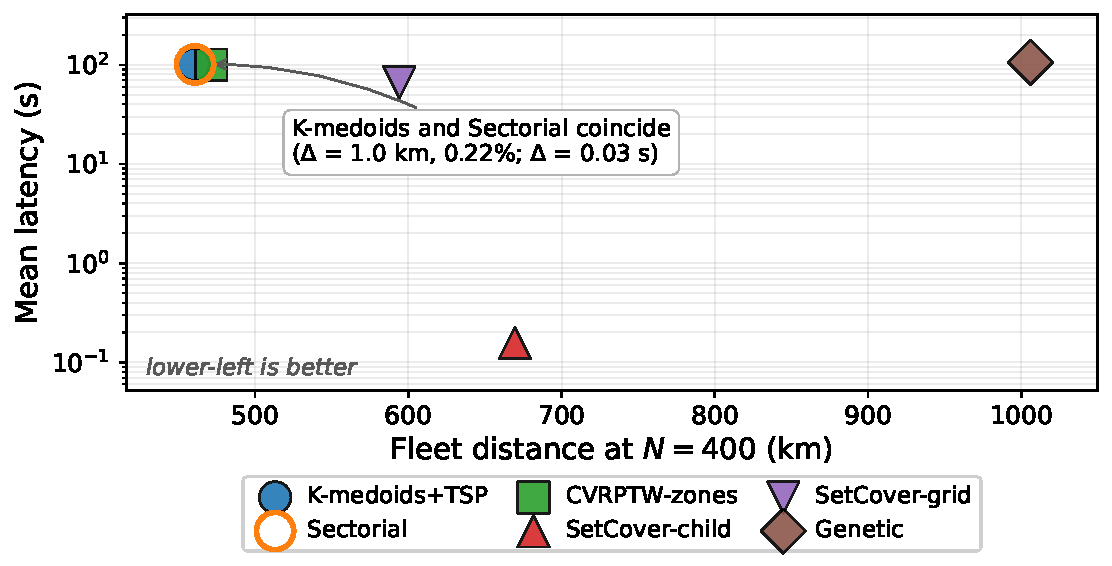
\includegraphics[width=\textwidth]{figures/pareto_N400.pdf}
  \caption{Distance--latency trade-off at $N{=}400$ (lower-left is
  better). The two leaders are all but coincident---differing by
  $1.0$~km ($0.22\%$) and $0.03$~s---so Sectorial is drawn as a hollow
  ring over the filled K-medoids marker rather than hidden beneath it,
  and the annotation reports the measured gap.}
  \label{fig:pareto}
\end{minipage}
\end{figure}

\begin{figure}[t]
\centering
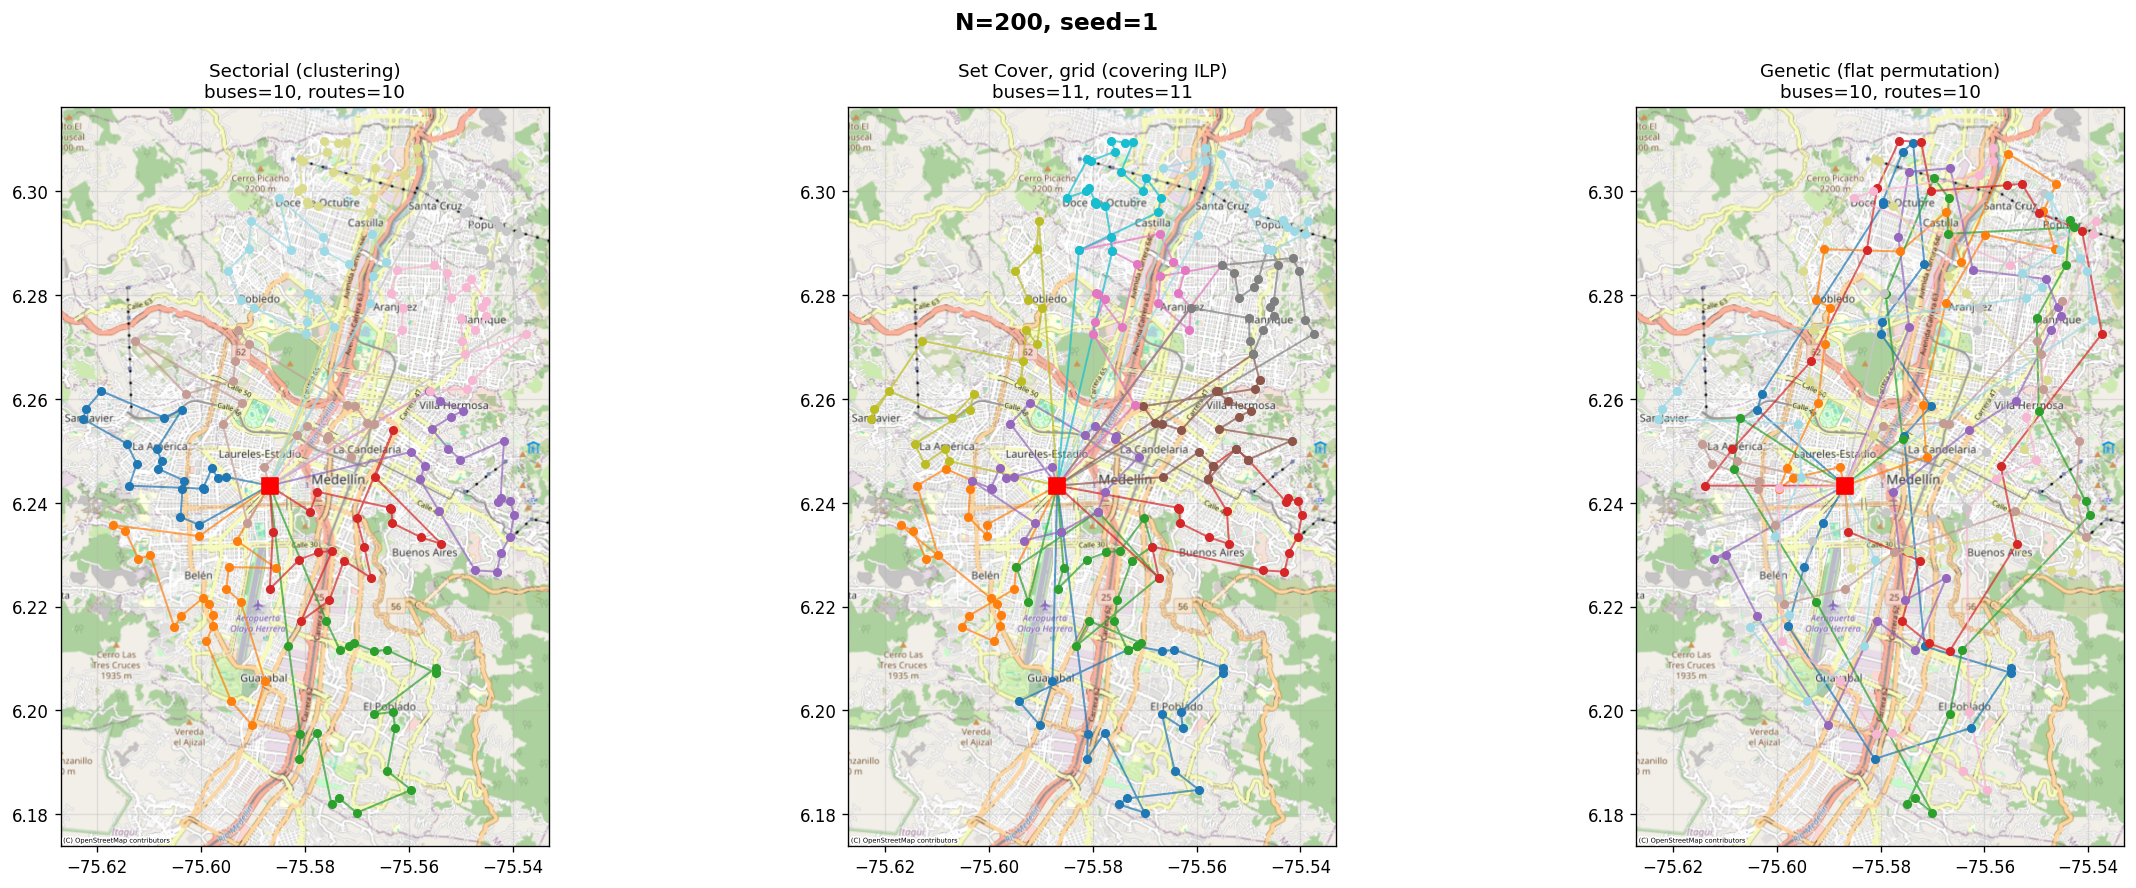
\includegraphics[width=0.95\textwidth]{figures/comparison_row_N200.png}
\caption{One representative of each solution paradigm on a shared
scenario ($N{=}200$, seed 1). Left: Sectorial produces compact,
wedge-shaped clusters radiating from the depot. Centre: the grid
set-covering ILP fills every selected route to capacity, so its routes
overlap and some students are visited twice. Right: the flat genetic
encoding interleaves geographically distant students in the same bus,
which is what its negative silhouette measures.}
\label{fig:grid}
\end{figure}

% =====================================================================
\section{Discussion}\label{sec:discussion}
% =====================================================================
\paragraph{Why clustering wins.}
K-medoids and Sectorial achieve the shortest fleet distance because
they produce spatially compact, well-separated clusters: at $N=400$
K-medoids attains the highest silhouette at $N=400$ ($0.276$;
Table~\ref{tab:quality}), though the zonal CVRPTW ($0.272$) is
statistically level with Sectorial ($0.266$), so cohesion alone does not
single out the two leaders. Cohesion also predicts cost only at scale:
within a density, silhouette correlates with fleet distance at
$r=-0.95$ at $N{=}400$ but merely $r=-0.02$ at $N{=}50$. Compact clusters shorten the inter-stop
distances the per-cluster TSP must traverse, so a good partition does
most of the optimization before routing begins, confirming the
cluster-first, route-second
rationale~\cite{CakirRevisitingProblem,Comert2018AStudy}. Notably, the cheap
angular score (Eq.~\ref{eq:sectorial-score}) recovers essentially the
quality of medoid optimization (Wilcoxon $p=0.36$); the $1.0$~km that
separates them at $N{=}400$ is well inside seed noise.

\paragraph{Why the genetic algorithm degrades.}
The genetic algorithm is competitive at $N=50$ ($115$ km) but collapses
at $N=400$ ($1006$ km, more than double the leaders) with a
\emph{negative} silhouette, indicating dispersed, interleaved clusters.
The cause is structural: a flat permutation encoding with a positional
capacity-chunk decoder has no notion of spatial locality, so the search
space grows as $n!$ while crossover and mutation routinely place
geographically distant students in the same bus. Within a fixed
generation budget the population cannot explore enough of this space,
and the myopic decoder cannot repair the damage. This reproduces a
well-known lesson from the VRP metaheuristic
literature~\cite{Baranwal2016DAVRPTW,Hatamlou2018BlackHole}: a
topology-agnostic \emph{representation} needs either far larger budgets
or locality-aware operators (e.g.\ cluster-based encodings or a
stronger local search such as
Lin--Kernighan~\cite{HelsgaunAnHeuristic}) to be competitive.

The scope of this result is narrow by construction: it indicts one
configuration---flat permutation chromosome, positional capacity-chunk
decoder, single 2-opt pass---not metaheuristic search in general.
Cluster-based chromosomes, repair operators, adaptive
large-neighbourhood search and learned construction
policies~\cite{Wu2024NCOSurvey} all target exactly the locality deficit
we observe, and none is tested here.

\paragraph{The CVRPTW trade-off.}
The zonal CVRPTW yields competitive distances but is not free: it
leaves up to ${\sim}1\%$ of students unserved when the $75$-minute
duration limit binds, and it uses more buses than the optimum
($22.4$ vs.\ $20$ at $N=400$). In exchange it produces by far the most
\emph{balanced} routes---its longest route ($30.3$ km) is
$33$--$62\%$ shorter than any other method's
(Table~\ref{tab:quality})---because the span-balancing penalty and the
explicit time dimension cap individual ride times. Where bounded
student ride time is a hard requirement, this is the only strategy that
delivers it directly.

\paragraph{Set covering: speed at a price.}
The set-cover programs are the speed champions: the per-child variant
solves every instance in under a quarter of a second. The price is route quality
(rank $5.45$ on distance) and fleet size ($26.9$ buses at $N=400$),
because greedily seeded candidate routes are far from distance-optimal.
The grid variant trades some of this speed for better distance, but its
latency becomes erratic at $N=400$ ($66.6\pm34.7$~s) as the candidate
pool---and hence the integer program---grows. These methods are the
right choice when a feasible plan is needed in near-real-time, e.g.\ for
interactive what-if analysis.

\paragraph{Limitations.}
Eleven seeds per density give $44$ blocks, which separate $11$ of the
$15$ pairs. We do not read the other four as equivalences: K-medoids
versus Sectorial is a genuine tie by every test we applied, whereas the
three trailing methods are simply too close to one another for this
design to order them.

More consequential is the absence of an external reference point. All six
strategies are our own implementations on instances we generate, so the
study establishes \emph{relative} standings under identical conditions
but calibrates them against neither published SBRP benchmark instances
nor a state-of-the-art metaheuristic such as adaptive large-neighbourhood
or tabu search; absolute quality therefore remains open, and closing this
gap is the highest-priority extension. Finally, the benchmark models a
single school with static demand and a homogeneous fleet, and all
strategies share one OR-Tools budget, so absolute latencies reflect that
budget rather than an intrinsic bound.

% =====================================================================
\section{Conclusions}\label{sec:conclusions}
% =====================================================================
We presented a unified, road-network-grounded benchmark of six SBRP
solution strategies evaluated on identical scenarios under a common
solver interface, with a formal model per strategy, complexity
validated against measured timings, and non-parametric statistical
testing. The central finding is clear
and statistically supported: under full coverage, capacitated
k-medoids and a multi-objective sectorial clustering are tied for the
shortest fleet distance and dominate the alternatives, because both
build compact clusters that make the downstream TSP easy. Set-covering
integer programs occupy the opposite corner of the trade-off---near
instant but with longer routes and larger fleets---while a zonal
CVRPTW is the method of choice when bounded ride time is mandatory. The
genetic algorithm we test is not competitive at scale; because that
configuration is deliberately naive, the result should be read as
evidence that a flat permutation encoding is a poor default for SBRP,
not as a verdict on metaheuristics with locality-aware operators.

Future work will (i)~calibrate the harness against published SBRP and
CVRP benchmark instances and against a state-of-the-art metaheuristic
baseline, which is the main gap in the present study;
(ii)~broaden the statistical design with more seeds to resolve the pairs
the Nemenyi test leaves open; (iii)~hybridize the genetic algorithm with
a cluster-based encoding and Lin--Kernighan local search;
(iv)~extend the harness to multi-school and dynamic-demand variants; and
(v)~convert the vehicle-kilometre results into emissions and operating
cost using fleet-specific factors, so that solver selection can be
argued directly in the sustainability terms that motivate it.

\subsubsection{Use of generative AI.}
Generative AI assisted with drafting and copy-editing the text, with the
scripts that compute the reported statistics and render the figures from the
benchmark output, and with literature search. It did not generate experimental
results: every reported number is the output of the described code run on the
described instances, and the authors verified all numbers, figures and
references against the underlying data and primary sources. The authors assume
full responsibility for the content of this paper.

\bibliographystyle{splncs04}
\bibliography{refs}

\end{document}
